% -*- root: ../ProjectPlan.tex -*-
\section{Time estimation and Schedule}
\label{secTimeEstimation}
\subsection{Gantt diagram}

This is the old Gantt diagram that is still quite useful. We don't consider important to update the gantt diagram because the changes made are minor changes, just some requirements removed to reduce timing.

\begin{figure}[hbtp]
\centering
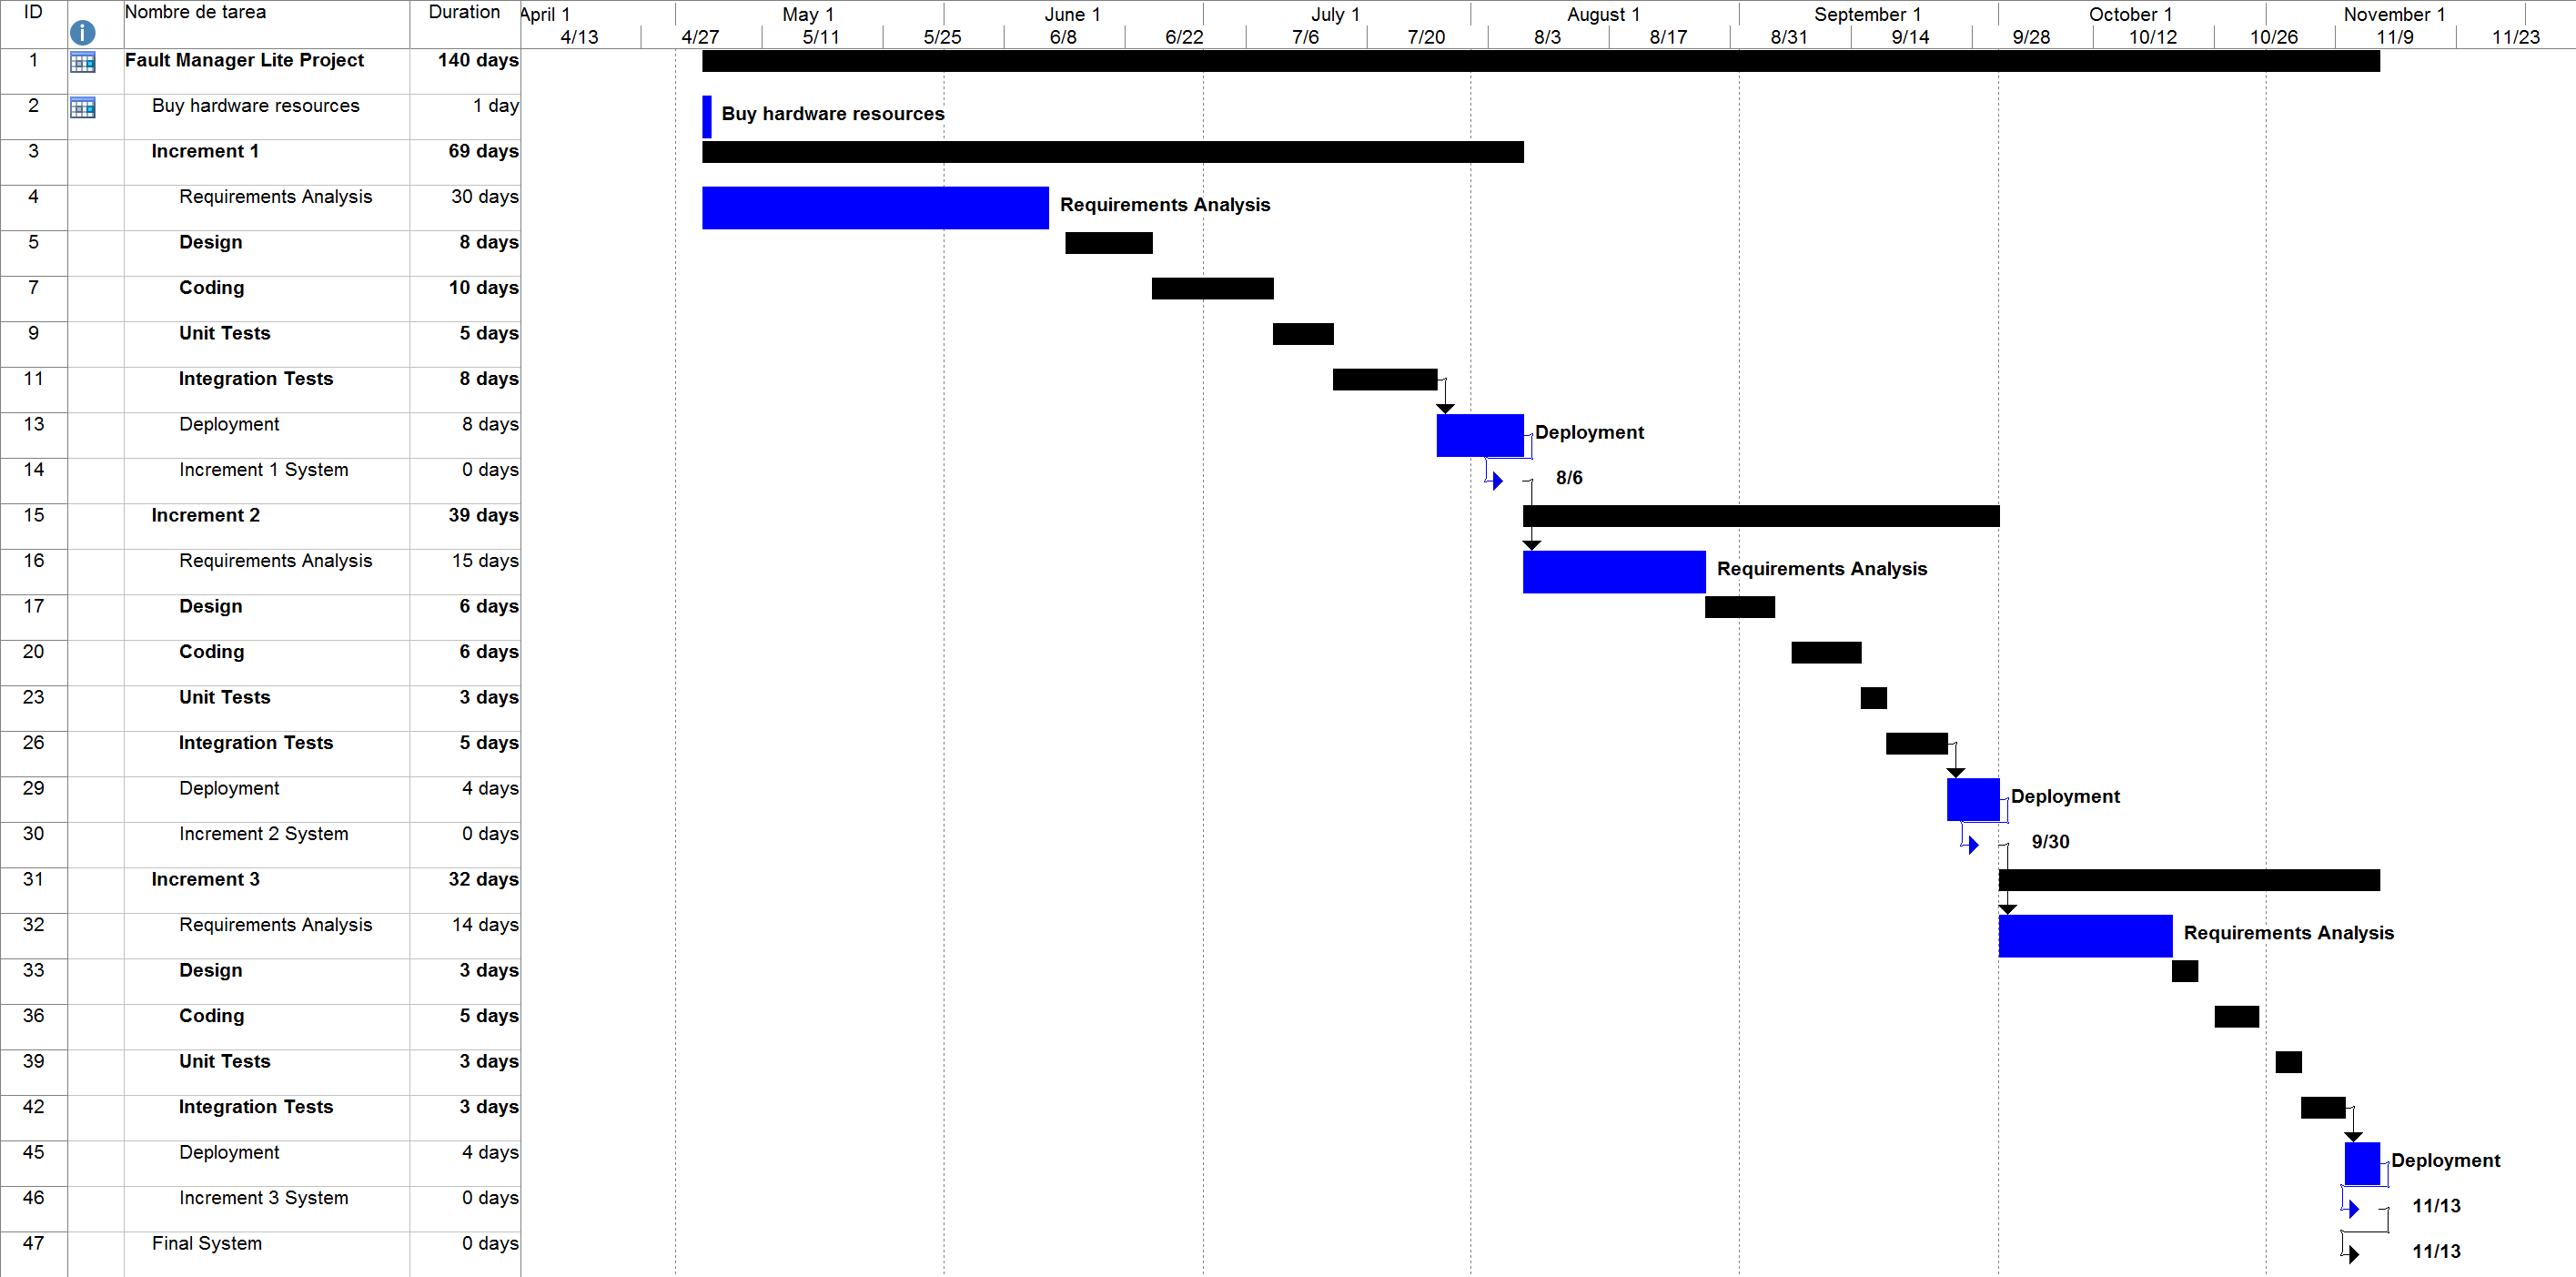
\includegraphics[width=0.8\textwidth]{img/GanttDiagram.png}
\caption{Simplified Gantt diagram.}
\label{figGanttSimple}
\end{figure}

Figure \ref{figGanttSimple} shows a simplified view of the Gantt diagram that represents the schedule of the project. A detailed version of this diagram is included in appendix \ref{chapGantt}.

\subsection{Increment planning}

We have decided to break down the development in 3 increments, each one dedicated to various subsystems. The details of the function points assigned to each increment and the corresponding effort is detailed in table \ref{tblIncrementsSubsystems}. Table \ref{tblSubsystemsAssignedIncrement} reflects the increment in which each subsystem will be completed and the corresponding percentage of each increment's effort dedicated to it.

This is the old detailed estimation of effort in terms of function points.

\begin{table}[hbtp]
\centering
\begin{tabular}{c|l|c|c}
\textbf{Increment} & \textbf{Subsystems} & \textbf{Function Points} & \textbf{Effort (person-days)} \\ \hline
Increment 1 & Task management & 102.3 & 149.972 \\
Increment 2 & Report System, Fault History & 50.6 & 74.213 \\
Increment 3 & Notification and Messaging & 48.4 & 70.986 \\ \hline
\textit{Total} &  & \textit{201.3} & \textit{295.106} \\
\end{tabular}

\caption{Detail of the old increments and corresponding effort.}
\label{tblIncrementsSubsystems}
\end{table}


As the time we had has been limited (10\% less than our initial estimation), we had to remove some system's functionalities. As a result of that process, we have obtained this new detailed estimation of effort in terms of function points.

\begin{table}[hbtp]
\centering

\begin{tabular}{c|l|c|c}
\textbf{Increment} & \textbf{Subsystems} & \textbf{Function Points} & \textbf{Effort (person-days)} \\ \hline
Increment 1 & Task management & 94.6 & 138.6836 \\
Increment 2 & Report System, Fault History & 48.4 & 70.9544 \\
Increment 3 & Notification and Messaging & 37.4 & 54.8284 \\ \hline
\textit{Total} &  & \textit{180.40} & \textit{264.47} \\
\end{tabular}
\caption{Detail of the new increments and corresponding effort.}
\label{tblIncrementsSubsystems}
\end{table}

As we can see in the efforts of each subsystems, they have changed. We have 10\% function points less, so we will finish 10\% earlier. The removed functionalities belonged principally to the messaging module and to the statistics module, the ones we thought that there were more dispensable.

The \textbf{removed requirements are} 

\begin{itemize}
\item Messaging module:
\subitem[21] Send messages to users.
\subitem[22] Read messages of a selected report.
\item Statistics:
\subitem[36] Generate statistics about incidences. (This requirement was just simplified to include less functionalities)
\subitem[37] Generate PDF file from report.
\item Fault system report
\subitem[26] See fault history (Even this requirement is removed, the functionality can be achieved by listing all reports (requirement 32) and check history of a reported fault (requirement 29)).
\end{itemize}



In table \ref{tblSubsystemsAssignedIncrement} one can see the effort for each subsystem, and one can corroborate that the affected ones are messaging and statistics.

\begin{table}[hbtp]
\centering

\begin{tabular}{l|c|c}
\textbf{Subsystem} & \textbf{Increment} & \textbf{Effort \%}  \\ \hline
Task Management & 1 & 100 \% \\
Reporting & 2 & 40 \% \\
Notification and Messaging & 2 & 60 \% \\
User Management & 3 & 29 \% \\
Faults History and Stats & 3 & 71 \% \\
\end{tabular}

\caption{Assigned increment and effort for each subsystem.}
\label{tblSubsystemsAssignedIncrement}
\end{table}

Now we include the effort for each phase of each increment in the table \ref{tblIncrementPhases} with its corresponding new effort.

\begin{table}[hbtp]
\centering

\begin{tabular}{|c|c|c|c|}
\hline
\textbf{Increment} & \textbf{Phase} & \textbf{Effort \%} & \textbf{Effort (person-days)} \\ \hline \hline

\multirow{7}{*}{\textsc{Increment 1}} & Analysis & 20 \% & 27.6 \\ \cline{2-4}
& Design & 20 \% & 27.6 \\ \cline{2-4}
& Coding & 20 \% & 27.6 \\ \cline{2-4}
& Unit tests & 10 \% & 13.8 \\ \cline{2-4}
& Integration tests & 20 \% & 27.6 \\ \cline{2-4}
& Implementation & 10 \% & 13.8 \\ \cline{2-4}
& \textit{Total} & \textit{100\%} & \textit{138.6836} \\ \hline \hline

\multirow{7}{*}{\textsc{Increment 2}} & Analysis & 20 \% & 14.20 \\ \cline{2-4}
& Design & 20 \% & 14.20 \\ \cline{2-4}
& Coding & 20 \% & 14.20 \\ \cline{2-4}
& Unit tests & 10 \% & 7.1 \\ \cline{2-4}
& Integration tests & 20 \% & 14.20 \\ \cline{2-4}
& Implementation & 10 \% & 7.1 \\ \cline{2-4}
& \textit{Total} & \textit{100\%} & \textit{70.9544} \\ \hline \hline

\multirow{7}{*}{\textsc{Increment 2}} & Analysis & 20 \% & 10.96 \\ \cline{2-4}
& Design & 20 \% & 10.96 \\ \cline{2-4}
& Coding & 20 \% & 10.96 \\ \cline{2-4}
& Unit tests & 10 \% & 5.4820 \\ \cline{2-4}
& Integration tests & 20 \% & 10.96 \\ \cline{2-4}
& Implementation & 10 \% & 5.4820 \\ \cline{2-4}
& \textit{Total} & \textit{100\%} & \textit{54.8284} \\ \hline

\end{tabular}

\caption{Detail of the increments with the corresponding phases for each one.}
\label{tblIncrementPhases}
\end{table}